\documentclass[fleqn,a4paper,12pt]{article}
\usepackage{standalone}		% Zum Einlesen aus anderen .tex-Files
\usepackage{geometry}		% Zur Bearbeitung des Layouts (Ränder,...)
\geometry{left=30mm, right=40mm, bottom=30mm}
\usepackage[german]{babel}
\usepackage[utf8]{inputenc}
\usepackage{amsmath}		% Mathematische Symbole
\usepackage{amssymb}     	% Nochmehr mathematische Symbole
\usepackage{dsfont}      	% Schriftsatz fuer Zahlenmengensymbole
%\usepackage{verbatim}   	% erweiterte Verbatim-Umgebung
\usepackage{alltt}       	% Quasi-Verbatim-Umgebung
\usepackage{fancyhdr}    	% Eigene Kopfzeilen
\usepackage{graphicx}    	% Zum Einbinden von Grafiken
% Einbinden einer eps-Grafik geht so: includegraphics{path}
\usepackage{wrapfig}
\usepackage{lscape}
\usepackage{rotating}
\usepackage{epstopdf}

% Skalierung der Grafiken
\setlength{\unitlength}{1cm}

\pagestyle{fancy}            % Eigene Kopfzeilen verwenden
\frenchspacing               % Kein Extrafreiraum nach Satzzeichen
\setlength{\parindent}{0pt}  % Neue Absaetze nicht einruecken
%\sloppy                     % Schlampige Absatzformatierung
\fussy                       % Penible Absatzformatierung
\linespread{1.5}             % Zeilenabstand

%andere Definitionen
\newcommand{\R}{{\mathbb R}}
\newcommand{\N}{{\mathbb N}}
\newcommand{\Z}{{\mathbb Z}}
\newcommand{\Q}{{\mathbb Q}}
\newcommand{\C}{{\mathbb C}}
\newcommand{\F}{\mathcal{F}}
\newcommand{\less}{\setminus}
\newcommand{\inv}{{}^{-1}}
\newcommand{\Land}{\bigwedge}
\newcommand{\Lor}{\bigvee}

\begin{document}
	"Ubungsaufgabe 11:\newline
	
	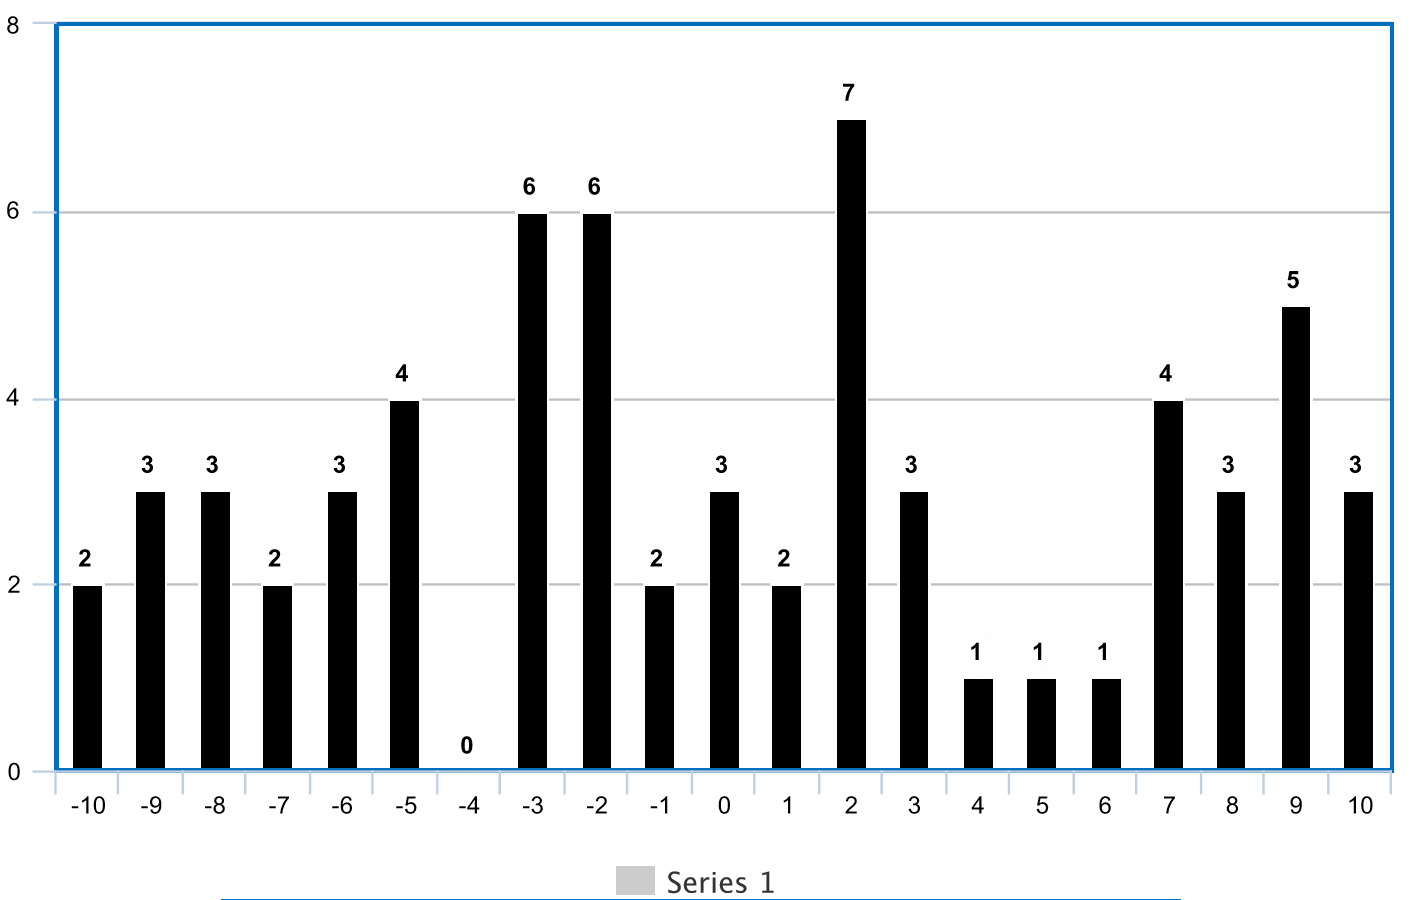
\includegraphics[scale=0.4]{H2}
	
	a)Ganzes Signal:\\
	$m_1 = 0,19		z_2 = 35$ \hspace{1cm}
	Median = 0,	Modalwerte: -4 und 2
	
	Signal in zwei H\"alften:\\
	Erste H\"alfte:	\hspace{5cm}										Zweite H\"alfte:\\
	$m_1 = 0,219$  $z_2 = 25$	\hspace{4cm}								$m_1 = -0,157$  $z_2 = 24$\\
	\\
	b)\\
	Es K\"onnen 16 nicht \"uberlappende Episoden heraugeschnitten werden.
	Episodemittelswertvektor: $m = \frac{1}{M}\sum_{i=0}^{M-1}e_i$\\
	$m = (-2,94, 1,38, 1,25, 1,06)^T$\\
	Keiner der Scharmittelwerte entspricht m1 $\rightarrow$ Signal ist weder station\"ar noch ergodisch.
	\newpage
	Kovarianzmatrix: $S = \frac{1}{M}\sum_{i=0}^{M-1}(e_i-m)(e_i-m)^T$\\
	$
	\begin{bmatrix}
	21   & -6,3 & 1,4	 &  -1,8 \\
	-6,3 & 44 	& -18	 &  -8 \\
	1,4  & -18	& 29 	 & -4,3 \\
	-1,8 & -8 	& -4,3	 &  34
	\end{bmatrix}
	$\\
	Korrelationsmatrix $R_{u,v} = \frac{S_{u,v}}{\sqrt{S_{u,v} \sqrt{S_{u,v}}}}$
	$
	\begin{bmatrix}
	1   & -0,21 & 0,06	 &  -0,07 \\
	-0,21 & 1 	& -0,5	 &  -0,21 \\
	0,06  & -0,5	& 1 	 & -0,14 \\
	-0,07 & -0,21 	& -0,14	 &  1
	\end{bmatrix}
	$\\Die Werte abseits der Hauptdiagonale sind (im Betrag) klein, $\rightarrow$ das Signal ist zuf\"allig\\
\end{document}